\documentclass[11pt,letterpaper]{article}

\usepackage[T1]{fontenc}
\usepackage[utf8]{inputenc}
\usepackage{lmodern}
\usepackage[margin=1in]{geometry}
\usepackage{microtype}
\usepackage{amsmath}
\usepackage{xcolor}
\usepackage{booktabs}
\usepackage{tabularx}
\usepackage{enumitem}
\usepackage{titlesec}
\usepackage{parskip}
\usepackage{tikz}
\usepackage[font=small,labelfont=bf]{caption}
\usepackage[hidelinks]{hyperref}

\definecolor{accent}{HTML}{3B6D11}
\definecolor{titledark}{HTML}{2C4A20}
\definecolor{muted}{HTML}{5F5E5A}
\definecolor{rulegray}{HTML}{C9C7BE}
\definecolor{wallgray}{HTML}{C9C7BE}
\definecolor{wallline}{HTML}{5F5E5A}
\definecolor{cavity}{HTML}{F5F4EF}
\definecolor{amberray}{HTML}{D98B0F}
\definecolor{leafgreen}{HTML}{97C459}
\definecolor{leafedge}{HTML}{3B6D11}

\titleformat{\section}{\normalfont\large\bfseries\color{accent}}{}{0pt}{}
\titlespacing*{\section}{0pt}{1.4em}{0.5em}

\newcommand{\Vcmax}{\ensuremath{V_{\mathrm{cmax}}}}
\newcommand{\Jmax}{\ensuremath{J_{\mathrm{max}}}}

\setlist[itemize]{leftmargin=1.4em, itemsep=0.35em, topsep=0.4em}

\tikzset{
  wall/.style={fill=wallgray, draw=wallline, line width=0.3pt},
  ray/.style={draw=amberray, line width=0.5pt, opacity=0.55, line cap=round},
  ray2/.style={draw=amberray, line width=0.4pt, opacity=0.32, line cap=round},
  beam/.style={draw=amberray, line width=1.6pt, line cap=round, -{Straight Barb[length=2mm]}},
  leader/.style={draw=muted, line width=0.3pt, dashed, dash pattern=on 2pt off 2pt},
  lbl/.style={font=\footnotesize, anchor=west, inner sep=1pt},
  lblc/.style={font=\footnotesize, anchor=north, inner sep=1pt, align=center},
}
\usetikzlibrary{arrows.meta}

\def\Rin{2.6}
\def\Rout{2.9}

\begin{document}

{\noindent\color{titledark}\LARGE\bfseries How an integrating sphere works\par}
\vspace{0.4em}
{\noindent\color{rulegray}\rule{\textwidth}{0.8pt}\par}
\vspace{0.5em}
{\noindent\color{muted}\itshape A hollow ball coated with a near-perfect white diffuser, whose job
is to scramble light until direction stops mattering.\par}
\vspace{1.2em}

\noindent An integrating sphere measures \emph{how much} light a sample sent back, regardless of
\emph{which way} it sent it. Every other design detail follows from that one requirement.

\begin{figure}[htbp]
\centering
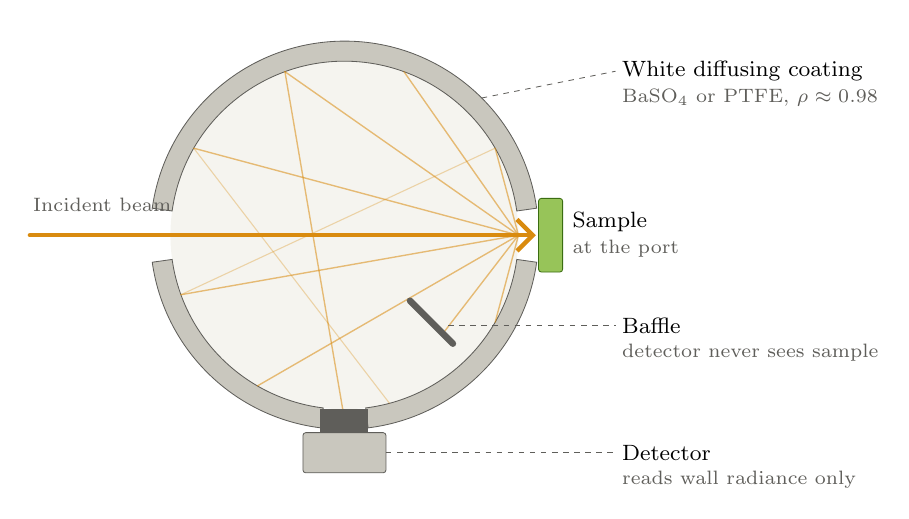
\begin{tikzpicture}[scale=0.85]

  \fill[cavity] (0,0) circle (\Rin);

  \filldraw[wall] (8:\Rout) arc[start angle=8, end angle=172, radius=\Rout]
      -- (172:\Rin) arc[start angle=172, end angle=8, radius=\Rin] -- cycle;
  \filldraw[wall] (188:\Rout) arc[start angle=188, end angle=263, radius=\Rout]
      -- (263:\Rin) arc[start angle=263, end angle=188, radius=\Rin] -- cycle;
  \filldraw[wall] (277:\Rout) arc[start angle=277, end angle=352, radius=\Rout]
      -- (352:\Rin) arc[start angle=352, end angle=277, radius=\Rin] -- cycle;

  \foreach \a in {30,70,110,150,200,240,330}
    \draw[ray] (\Rin,0) -- (\a:\Rin);
  \draw[ray] (\Rin,0) -- (1.47,-1.47);

  \draw[ray2] (150:\Rin) -- (285:\Rin);
  \draw[ray2] (30:\Rin) -- (200:\Rin);
  \draw[ray] (110:\Rin) -- (0,-2.75);

  \draw[wallline, line width=2.4pt, line cap=round] (0.98,-0.98) -- (1.62,-1.62);

  \filldraw[fill=wallline, draw=wallline] (-0.35,-2.95) rectangle (0.35,-2.6);
  \filldraw[fill=wallgray, draw=wallline, line width=0.3pt, rounded corners=1pt]
      (-0.62,-3.55) rectangle (0.62,-2.95);

  \draw[beam] (-4.7,0) -- (2.86,0);

  \filldraw[fill=leafgreen, draw=leafedge, line width=0.3pt, rounded corners=1pt]
      (\Rout,-0.55) rectangle ++(0.36,1.1);

  \draw[leader] (2.05,2.05) -- (4.05,2.45);
  \node[lbl] at (4.1,2.45) {White diffusing coating};
  \node[lbl, text=muted] at (4.1,2.05) {\scriptsize BaSO$_4$ or PTFE, $\rho \approx 0.98$};

  \node[lbl] at (3.36,0.2) {Sample};
  \node[lbl, text=muted] at (3.36,-0.2) {\scriptsize at the port};

  \draw[leader] (1.55,-1.35) -- (4.05,-1.35);
  \node[lbl] at (4.1,-1.35) {Baffle};
  \node[lbl, text=muted] at (4.1,-1.75) {\scriptsize detector never sees sample};

  \draw[leader] (0.62,-3.25) -- (4.05,-3.25);
  \node[lbl] at (4.1,-3.25) {Detector};
  \node[lbl, text=muted] at (4.1,-3.65) {\scriptsize reads wall radiance only};

  \node[lbl, text=muted] at (-4.7,0.45) {\scriptsize Incident beam};

\end{tikzpicture}
\caption{Cross-section in reflectance mode. The beam enters through a port, strikes the sample, and
scatters. Light bounces many times off the white coating before any of it reaches the detector,
which is shielded by a baffle so it sees only wall. For transmittance the sample moves to the
entrance port and a white plug fills the sample port; nothing else changes.}
\label{fig:sphere}
\end{figure}

\section{What is actually happening}

\textbf{The coating does the work.} The inside is coated with a highly Lambertian, highly reflective
diffuser --- pressed barium sulfate (BaSO$_4$) or sintered PTFE (Spectralon). Two properties matter:
reflectance $\rho$ is very high, typically $0.95$ to $0.99$ across $350$--$2500$\,nm, and the
scattering is Lambertian, meaning reflected radiance is the same in every direction regardless of
how the light arrived.

\textbf{Multiple bounces destroy directional information.} A photon entering the cavity hits the
wall, scatters, hits again, scatters again --- typically dozens of times before it is absorbed or
escapes through a port. After a handful of bounces, the memory of its original direction is gone.
Wall radiance becomes uniform everywhere, and proportional to the \emph{total} flux that entered,
not to its angular distribution. That is the ``integrating'' in the name.

The sphere multiplier quantifies it:
\begin{equation}
  M = \frac{\rho}{1 - \rho\,(1-f)}
  \label{eq:multiplier}
\end{equation}
where $f$ is the port fraction, the total port area divided by the sphere's inner surface area. With
$\rho = 0.98$ and $f = 0.02$, $M \approx 25$: light accumulates about twenty-five passes' worth of
wall interaction before leaving. Drop $\rho$ to $0.94$ and $M$ falls to roughly $12$. This is why
coating contamination is so damaging --- the relationship is strongly nonlinear, and it is
wavelength-dependent, since both PTFE and BaSO$_4$ lose reflectance beyond about $2200$\,nm.

\textbf{The baffle is not optional.} If the detector could see the sample port directly, it would
preferentially weight light that happened to leave the sample in that one direction --- exactly the
bias the sphere exists to remove. The baffle forces the detector to see only wall, never sample. The
same logic applies to the entrance port: the detector must not see the first-bounce spot either.

\textbf{Ports are the loss term.} Every opening is a hole in an otherwise perfect diffuser. Keep the
total port fraction below about $5\%$; above that, throughput collapses and the sphere stops being
spatially uniform.

\section{Why a sphere rather than a detector}

A leaf scatters light in every direction, and not evenly. Point a bare detector at one angle and you
sample a narrow, biased slice of what came off. The sphere removes the problem geometrically rather
than by modelling it (Figure~\ref{fig:why}).

\begin{figure}[htbp]
\centering
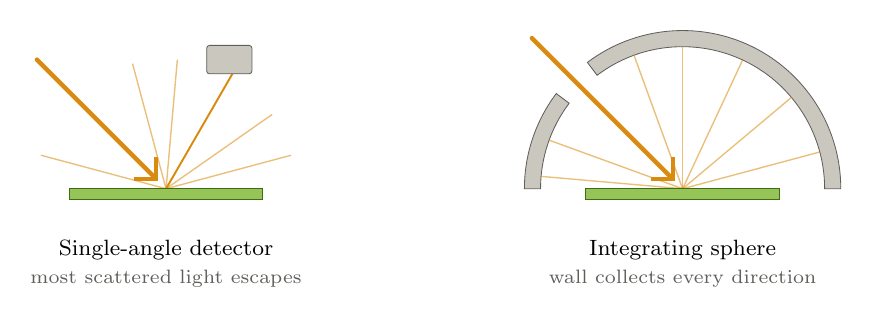
\begin{tikzpicture}[scale=0.82]

  \foreach \a in {15,35,85,105,165}
    \draw[ray] (0,0) -- (\a:2.0);
  \draw[draw=amberray, line width=0.7pt, line cap=round] (0,0) -- (60:2.06);
  \filldraw[fill=wallgray, draw=wallline, line width=0.3pt, rounded corners=1pt]
      (0.63,1.78) rectangle (1.33,2.22);
  \draw[beam] (-2.0,2.0) -- (-0.12,0.12);
  \filldraw[fill=leafgreen, draw=leafedge, line width=0.3pt] (-1.5,-0.16) rectangle (1.5,0);
  \node[lblc] at (0,-0.75) {Single-angle detector};
  \node[lblc, text=muted] at (0,-1.2) {\scriptsize most scattered light escapes};

  \begin{scope}[xshift=8cm]
    \filldraw[wall] (0:2.45) arc[start angle=0, end angle=127, radius=2.45]
        -- (127:2.2) arc[start angle=127, end angle=0, radius=2.2] -- cycle;
    \filldraw[wall] (143:2.45) arc[start angle=143, end angle=180, radius=2.45]
        -- (180:2.2) arc[start angle=180, end angle=143, radius=2.2] -- cycle;
    \foreach \a in {15,40,65,90,110,160,175}
      \draw[ray] (0,0) -- (\a:2.2);
    \draw[beam] (135:3.3) -- (135:0.16);
    \filldraw[fill=leafgreen, draw=leafedge, line width=0.3pt] (-1.5,-0.16) rectangle (1.5,0);
    \node[lblc] at (0,-0.75) {Integrating sphere};
    \node[lblc, text=muted] at (0,-1.2) {\scriptsize wall collects every direction};
  \end{scope}

\end{tikzpicture}
\caption{The same scattering surface, measured two ways. A detector at a single viewing angle
intercepts one direction out of the full hemisphere, so the reading depends on the sample's
bidirectional reflectance distribution. The spherical wall intercepts all of them.}
\label{fig:why}
\end{figure}

\section{Reflectance and transmittance}

The measurement is always a ratio of two sphere readings taken under identical geometry:
\begin{equation}
  R = \frac{S_{\mathrm{sample}} - S_{\mathrm{dark}}}
           {S_{\mathrm{reference}} - S_{\mathrm{dark}}} \times R_{\mathrm{std}}
  \label{eq:ratio}
\end{equation}

For reflectance, the reference is a calibrated white standard at the same port. For transmittance,
the reference is the beam entering the empty sphere with nothing in the path. Because the same wall,
the same detector, and the same baffle serve both measurements, the two are directly comparable ---
which is what lets you compute leaf absorptance:
\begin{equation}
  A(\lambda) = 1 - R(\lambda) - T(\lambda)
  \label{eq:absorptance}
\end{equation}

\noindent without ever measuring absorbed energy directly. For a healthy leaf this gives the
familiar picture: $A \approx 0.85$--$0.90$ through the visible, where pigments absorb; collapsing to
$A \approx 0.05$--$0.10$ across the near-infrared plateau, where light is scattered by mesophyll cell
walls rather than absorbed; then rising again at the water bands near $1450$ and $1940$\,nm.

\section{Two error sources worth knowing about}

\begin{itemize}
  \item \textbf{Substitution error.} When the sample replaces the white standard at the port, it
        changes the sphere's average wall reflectance. A dark leaf at the port lowers $M$ in
        Equation~\eqref{eq:multiplier} relative to the white reference, so the measured ratio is
        biased. Dual-beam and comparison-mode spheres, where sample and reference are both
        permanently mounted and the beam alternates between them, cancel this; single-beam
        substitution spheres do not. The error is largest for strongly absorbing samples, so it hits
        visible-region chlorophyll measurements hardest.
  \item \textbf{The wall uniformity assumption.} The derivation assumes the detector sees a wall
        patch whose radiance represents the whole cavity. Ports, baffles, and any coating damage
        break that. A scratched or yellowed sphere produces wavelength-dependent errors that look
        exactly like real spectral features.
\end{itemize}

\section{For hyperspectral trait modelling}

Integrating-sphere leaf spectra are the closest thing available to a ground truth for leaf optical
properties, which is why models for nitrogen, LMA, chlorophyll, and carotenoids calibrate so well on
them. But different spheres --- the LI-COR 6800 integrating sphere, the ASD RTS-3ZC, a Cary with an
internal diffuse reflectance accessory --- have different port fractions, different baffling, and
different substitution-error behaviour. Cross-instrument transfer of PLSR coefficients is genuinely
hard, and the residual is usually instrument geometry rather than chemistry.

Having both $R$ and $T$, and hence $A$, is a real advantage for the structural and biochemical
traits. Cellulose and lignin absorb in the shortwave infrared, where leaves also scatter strongly;
separating $R$ from $T$ lets you disentangle scattering from absorption in a way reflectance alone
cannot. If transmittance is available and only reflectance is going into the models, that is
information left on the table --- the PROSPECT-style inversion route for \Vcmax{} and \Jmax{} priors
in particular benefits from both.

\end{document}
